\documentclass{article}
\usepackage{amsmath, amssymb, cite, algorithmic, url, braket}
\usepackage{graphicx}
\usepackage{pythonhighlight}
\usepackage[margin=1.5cm]{geometry}
\usepackage[title]{appendix}
\usepackage{subfigure}
\usepackage{listings}
\usepackage{booktabs}

\graphicspath{{../pic/}}
\lstset{
language=[ANSI]{C},
showtabs=true,
tab=,
tabsize=2,
basicstyle=\ttfamily\footnotesize,%\setstretch{.5},
stringstyle=\color{stringcolour},
showstringspaces=false,
alsoletter={1234567890},
otherkeywords={\%, \}, \{, \&, \|},
keywordstyle=\color{keywordcolour}\bfseries,
upquote=true,
morecomment=[s]{/*}{*/},
commentstyle=\color{commentcolour}\slshape,
literate=*%
{=}{{\literatecolour=}}{1}%
{-}{{\literatecolour-}}{1}%
{+}{{\literatecolour+}}{1}%
{*}{{\literatecolour*}}{1}%
{!}{{\literatecolour!}}{1}%
{[}{{\literatecolour[}}{1}%
{]}{{\literatecolour]}}{1}%
{<}{{\literatecolour<}}{1}%
{>}{{\literatecolour>}}{1}%
% {>>>}{\pythonprompt}{3}%
,%
frame=trbl,
rulecolor=\color{black!40},
backgroundcolor=\color{white},
breakindent=.5\textwidth,frame=single,breaklines=true
}

\begin{document}
\title{DSP Monthly Project 02}
\author{Xu, Minhuan}
\maketitle
\tableofcontents
\begin{abstract}
In my first project, I deployed a web page to display the media stream captured by the Raspberry Pi camera, but that was completely modeled after the repository content on GitHub. What I want to do this time is to write some of my own code with the help of some python libraries. This time the function I want to achieve is not only to be able to get the photos taken by the Raspberry Pi, but also to be able to control the Raspberry Pi through the web page, perform the work of taking pictures or making the buzzer ring (warning visitors when I'm not there). At the same time, I will combine some ready-made facial recognition solutions to make it more in line with the original vision of the facial recognition surveillance camera in this project.
\end{abstract}

\section{Introduction}
In this project, I want my Raspberry Pi (Raspi) to take pictures and do face recognition under my control remotely\cite{webcontrol}. So I will host a web page which contains buttons which can control the Raspi, for example, tell the Raspi to take a photo and show it to you.

The things I will use contains: bottle, jQuery, openCV and GPIO on Raspi.
\paragraph*{bottle}
Bottle is a fast, simple and lightweight WSGI micro web-framework for Python. It is distributed as a single file module and has no dependencies other than the Python Standard Library. \cite{bottle-py}

\paragraph*{jQuery}
Combine with bottle, the methods in jQuery (GET, POST) make a link between the button in HTML and python script.
\paragraph*{GPIO}
Python can read and write the status and the value of the GPIO (General-purpose input/output) ,so that we can drive a buzzer or LED.

\begin{figure}[!h]
	\centering
	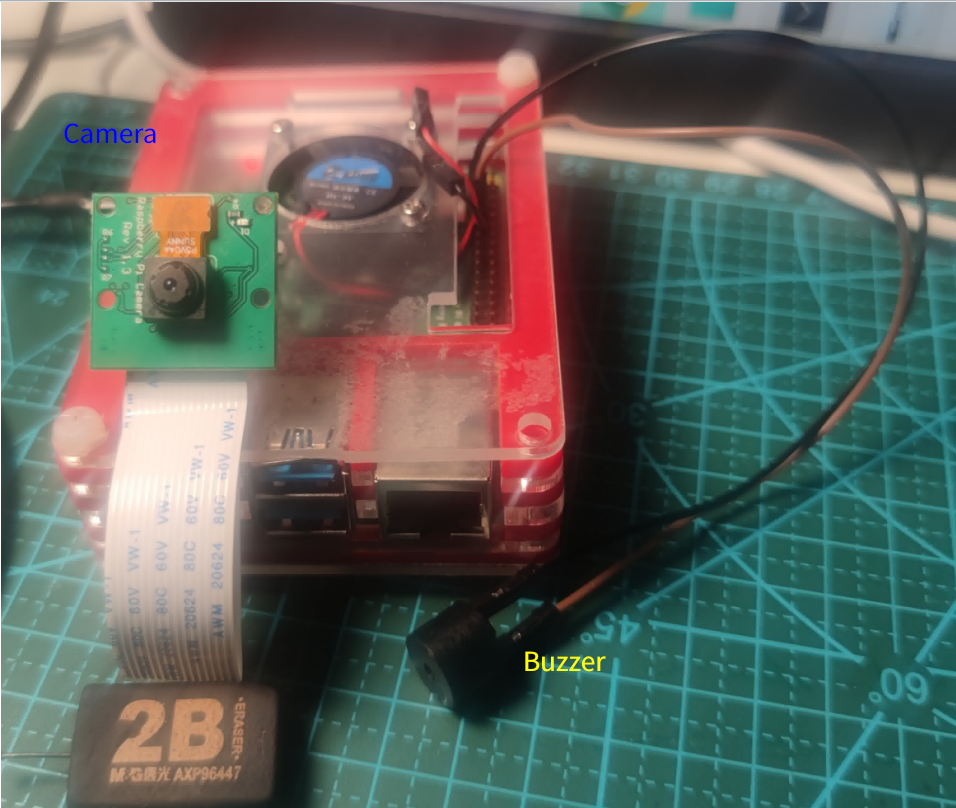
\includegraphics[width=2 in]{../pic/raspi-2.png}
	\caption{How My Raspberry Pi Looks Now}
	\label{fig:raspi-2}
\end{figure}

\newpage

\section{Web Page}
The HTTP protocol defines several request methods for different tasks. \verb|GET| is the default for all routes with no other method specified. These routes will match \verb|GET| requests only. To handle other methods such as \verb|POST|, \verb|PUT|, \verb|DELETE| or \verb|PATCH|, add a method keyword argument to the route() decorator or use one of the five alternative decorators: \verb|get()|, \verb|post()|, \verb|put()|, \verb|delete()| or \verb|patch()|. The \verb|POST| method is commonly used for HTML form submission.

For example, the \verb|@get('/')| decorator will let the function which is decorated by it run every time the user want to access the root of the site. To order return the browser with an \verb|index.html| file, we write \verb|return template('index')|

The source code of \verb|index.html| is zipped with this report. Have a see at how it looks like in Fig.~\ref{fig:webcontrol-page} . The buttons named like \verb|UP| are designed for a camera which can move up and down, left and right, so that the 4 buttons on the first line don't work now. The \verb|FETCH| button is used to take a new photo. The \verb|WARNING| button is used to let the buzzer beep for $1 ~\mathrm{s}$.

\begin{figure}[!h]
	\centering
	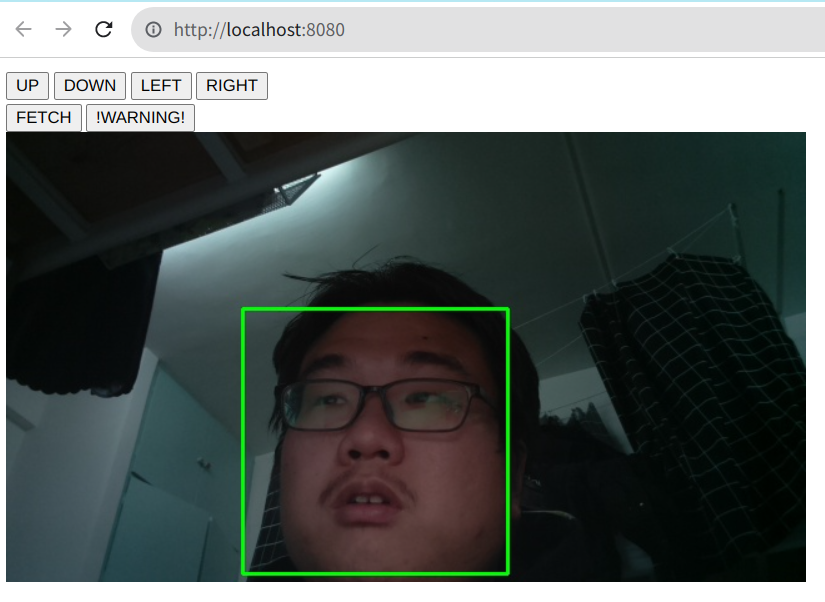
\includegraphics[width=2.5 in]{../pic/webcontrol-page.png}
	\caption{My Web Page Controlling the Raspi}
	\label{fig:webcontrol-page}
\end{figure}

\section{Face-Recognition}
Object Detection using Haar\cite{opencv} feature-based cascade classifiers is an effective object detection method proposed by Paul Viola and Michael Jones in their paper, "Rapid Object Detection using a Boosted Cascade of Simple Features" in 2001. It is a machine learning based approach where a cascade function is trained from a lot of positive and negative images. It is then used to detect objects in other images. Here we will work with face detection.

Haar cascade classifier works with a sliding window approach. So by applying a sliding window approach, you slide a window through out the picture than you resize it and search again until you can not resize it further. So with every iteration Haar's cascaded classifier true outputs are stored.  You can check what it detects by giving minNeighbors 0. 


So there are a lot of face detection because of resizing the sliding window and a lot of false positives too. So to eliminate false positives and get the proper face rectangle out of detection, neighborhood approach is applied. It is like if it is in neighborhood of other rectangles then it is OK, you can pass it further. So this number determines the how much neighborhood is required to pass it as a face rectangle. 

\begin{figure}[!h]
	\centering
	\subfigure[Giving minNeighbors 1]{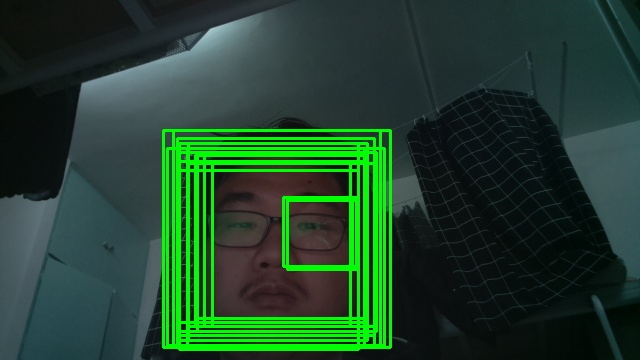
\includegraphics[height=1.5 in]{../pic/result1.jpg}}
	\hspace{0 pt}
	\subfigure[Giving minNeighbors 5]{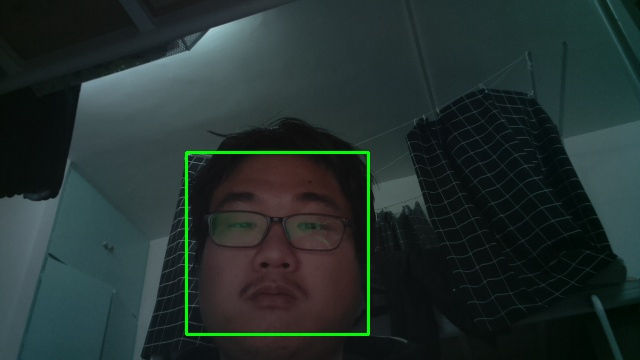
\includegraphics[height=1.5 in]{../pic/result2.jpg}}
	\caption{Modifying Parameters}
	\label{fig:results}
\end{figure}

\section{GPIO Control On Raspberry Pi}
Raspi has several programmable GPIO pins, any of them can be designated (in software) as an input or output pin and used for a wide range of purposes, see Fig.~\ref{fig:GPIO} (From Raspberry Pi Document\cite{GPIO}).

\begin{figure}[!h]
	\centering
	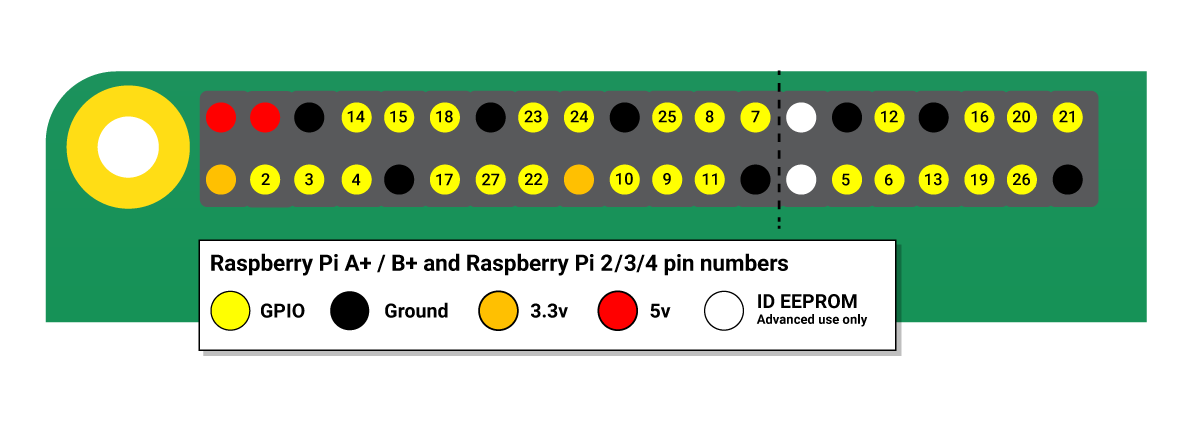
\includegraphics[width=3 in]{../pic/GPIO.png}
	\caption{GPIO Pins On Raspberry Pi}
	\label{fig:GPIO}
\end{figure}

The pin I used is the GPIO17 and the ground nearest. It is easy to control the voltage on the GPIO by python, so if the GPIO17 is $5 ~\mathrm{V}$, the buzzer will beep, or the GPIO17 is $0 ~\mathrm{V}$, the buzzer don't work.

\bibliographystyle{ieeetr}
\bibliography{../bib/database}

\begin{appendices}
\section{Code Listing}
\begin{python}
# host.py
from lib.bottle import run, get, post, static_file, template
from picam import fetch
from bell import warning

#init page
@get('/')
def index():
    return template('index')

#load picture for index page
@get('/<filename:re:.*\.jpg>')
def get_image(filename):
    return static_file(filename, root='./image', mimetype='image/jpg')

#For later use (camera go up, down, left, right)
@post('/<name:re:cam-[^.]+>')
def response(name):
    print(name)

#Tell the camera to take a photo, then judge if there's a face
@post('/fetch')
def picture():
    fetch()

#Remote control the buzzer to warn the stranger
@post('/warning')
def bell():
    warning()

#run this web server
run(host='0.0.0.0', port=8080)
\end{python}

\begin{python}
#picam.py
from picamera import PiCamera 
from time import sleep
import numpy as np
import cv2

def GetFace(imname):
    """
    use a simple built-in classifier of opencv, to recognize a face
    """
    image = cv2.imread(imname)
    face_cascade = cv2.CascadeClassifier('./lib/haarcascade_frontalface_alt.xml')
    gray = cv2.cvtColor(image, cv2.COLOR_BGR2GRAY)
    faces = face_cascade.detectMultiScale(gray, minNeighbors=5)
    for (x, y, w, h) in faces:
        cv2.rectangle(image, (x, y), (x+w, y+h), (0, 255, 0), 2)
    cv2.imwrite('./image/result2.jpg', image)
    if len(faces) != 0:
        print('Face!')
    else:
        print('No Face!')

def fetch():
    """
    take a photo and send it to the opencv recognition
    """
    camera = PiCamera()
    camera.resolution = (640, 360)
    camera.capture('./image/original.jpg')
    camera.close()
    GetFace(imname='./image/original.jpg')

GetFace(imname='./image/original.jpg')
\end{python}

\begin{python}
# bell.py
import RPi.GPIO as GPIO
import time

def warning():
    fm = 11
    GPIO.setmode(GPIO.BOARD) # use the physical number on the raspi
    GPIO.setup(fm, GPIO.OUT, initial=GPIO.LOW) # initially low (disable)

    GPIO.output(fm, GPIO.HIGH)
    time.sleep(0.1)
    GPIO.output(fm, GPIO.LOW) # run for 1 second
    GPIO.cleanup()            # clearup the status of the port
    print('Warning!!')        # warning in the terminal as well
\end{python}

\begin{lstlisting}
<!DOCTYPE html>
<html lang="en">
<head>
    <meta charset="UTF-8">
    <meta name="viewport" content="width=device-width, initial-scale=1.0">
    <title>Remote Raspi</title>
    <script src="http://code.jquery.com/jquery.js"></script>
    <script>
        $(function(){
            $("button").click(function(){
                location.replace(location)
                $.post(this.id);
            });
        });
    </script>
</head>

<body>
        <button id='cam-up' type="button">UP</button>
        <button id='cam-down' type="button">DOWN</button>
        <button id='cam-left' type="button">LEFT</button>
        <button id='cam-right' type="button">RIGHT</button>
        <br>
        <button id='fetch' type="button">FETCH</button>
        <button id='warning' type="button">!WARNING!</button>
        <br>
        <img src="result.jpg">
</body>
</html>
\end{lstlisting}

\end{appendices}

\end{document}